%% Template para TCC do Curso de Ciência da Computação da Universidade Vila Velha
%% Editado por: Leonardo Muniz de Lima
%% Editado por: Sabrina Siqueira Panceri
%% Última Alteração: 10/05/2013

%==============================================================================
%								IMPORTANTE
%==============================================================================
% - As referências não funcionam no Windows.
% - Se vc preferir utilizar qq sistema operacional GNU/Linux em máquina virtual, poderá ter problemas com as referências.
% - Para um bom funcionamento deste modelo, aconselho que o mesmo seja utilizado em um sistema operacional GNU/Linux de sua preferência
% - Alguns editores LaTex possuem uma interface mais amigável, são eles: Kile, TexMaker, Lyx, etc.
% - Para gerar ou atualizar o sumário, as citações no texto, e as referências bibliográficas, compile o arquivo no mínimo 3 vezes. Se ocorrer um erro, exclua os arquivos gerados pela compilação e compile o arquivo .tex principal novamente. Há vezes em que a compilação não atualiza todos os arquivos.
% - Se ao compilar um arquivo ocorrer um erro, tente ler o erro e entender o que deu errado. 
%==============================================================================


%==============================================================================
%                              PREÂMBULO
%==============================================================================
\documentclass[brazil]{abnt-UVV/abnt-uvv}
\usepackage{tabularx}
\usepackage{graphicx,url, enumerate}
\usepackage[brazil]{babel}   
\usepackage[utf8]{inputenc}
\usepackage[T1]{fontenc}
\usepackage[colorlinks,linkcolor=black,citecolor=black, hyperindex]{hyperref}
\usepackage{listings}

\renewcommand{\rmdefault}{phv} 
\renewcommand{\sfdefault}{phv} 
\setcounter{secnumdepth}{3}
%==============================================================================

%==============================================================================
%                              ELEMENTOS PRÉ-TEXTUAIS
%==============================================================================
\autor{Thalles de Almeida Batista}

\titulo{Conversor de lógica estruturada textual para lógica estruturada gráfica}

\orientador[Orientador:]{Msc. Alessandro Bertolani de Oliveira}

\comentario{Trabalho de Conclusão de Curso apresentado a Universidade Vila Velha como requisito parcial para a obtenção do grau de Bacharel em Ciência da Computação.}

\instituicao{UNIVERSIDADE VILA VELHA \par CURSO DE CIÊNCIA DA COMPUTAÇÃO}

\local{VILA VELHA}

\data{2016} 
%==============================================================================

%INÍCIO DO DOCUMENTO
\begin{document} 

%============================
% 1) Capa
%===========================
\capa
%==============================================================================

%============================
% 2) Folha de Rosto
%===========================
\folhaderosto
%==============================================================================

%============================
% 3) Folha de Aprovacao
%===========================
\begin{folhadeaprovacao}
\begin{center}
\autorformat\ABNTautordata
\end{center}
\vspace{2cm}
\begin{center}
\tituloformat\ABNTtitulodata
\end{center}
\vspace{1.0cm}
\hspace{7cm}{\large\bf{BANCA EXAMINADORA}}
\assinatura{Prof. Msc. Alessandro Bertolani de Oliveira \par Universidade Vila Velha \par Orientador}
\assinatura{Prof. Msc. MEMBRO DA BANCA  \par Universidade Vila Velha}
\assinatura{Prof. Msc. MEMBRO DA BANCA  \par Universidade Vila Velha}
\vspace{1cm}
\termino{DD}{MM}{\ABNTdatadata} %DIA DA APRESENTAÇÃO
\end{folhadeaprovacao}
%==============================================================================

%==============================================================================
% 4) Folha de Autorização para publicação
% Obrigatória para TCC com nota final maior ou igual a 8.0 pontos.
%==============================================================================
Autorizo que a UVV, sem ônus, promova a publicação de minha monografia em página própria na Internet ou outro meio de divulgação de trabalho científico.

\vspace{2cm}
\hspace{7cm}{\large\bf{ASSINATURAS}}
\assinatura{Prof. Msc. Alessandro Bertolani de Oliveira \par Universidade Vila Velha \par Orientador}
\assinatura{Thalles de Almeida Batista \par Universidade Vila Velha}
\vspace{2cm}
DD/MM/AAAA %DIA DA APRESENTAÇÃO
\pagebreak
%==============================================================================

%==============================================================================
% 5) Dedicatória (Opcional)
%==============================================================================
\chapter*{DEDICATÓRIA}
 \vspace*{15cm}
 \begin{flushright}
 {\large {\em {SEU TEXTO \par SEU TEXTO \par SEU TEXTO}}}
\end{flushright}
\pagebreak
%=============================================================================


%==============================================================================
% 6) Agradecimentos (Opcional)
%==============================================================================
\chapter*{AGRADECIMENTOS}

SEU TEXTO. SE CITAR ALGUMA PESSOA, COLOQUE O NOME DELA COMPLETO.

\pagebreak
%=============================================================================

%=============================================================================
% 7) Epígrafe (Opcional)
%=============================================================================
\vspace*{15cm}
\begin{flushright}{}"\emph{SEU TEXTO.}"\\
{\small NOME DO AUTOR DA EPÍGRAFE}\end{flushright}{\small \par}
\vfill{}
\pagebreak
%=============================================================================

%=============================================================================
% 8) Lista de tabelas
%=============================================================================
\listadetabelas
%=============================================================================

%=============================================================================
% 9) Lista de figuras
%=============================================================================
\listadefiguras
%=============================================================================


%=============================================================================
% 10) Lista de siglas
%=============================================================================
\pretextualchapter{\listofabreviationsname}

\begin{tabbing}
\hspace{0.80cm}SIGLA \= espaço \= Significado da sigla que pode ser grande \kill
\hspace{0.80cm}EXEMPLO 		\> \> Descrição / significado\\ 
\end{tabbing}
%=============================================================================

%=======================
% 11) Sumário
%=======================
\sumario
%=============================================================================


%==================
% 11) Resumo
%==================
\begin{resumo} 
Resumo

\paragraph{Palavras-Chave:} Palavras.
\end{resumo}
%=============================================================================

%=============================================================================
% 12) Abstract (Não é necessário em TCC's somente em dissertações e teses.)
%=============================================================================
\begin{abstract}

\textit{ TEXT }

\paragraph{Keywords:} \textit{ WORDS }
\end{abstract}
%=============================================================================

%==============================================================================
%				  ELEMENTOS TEXTUAIS
%==============================================================================

%Inclusão dos capítulos que foram escritos em arquivos separados.
%Os capítulos são gerados de acordo com a ordem de inclusão.
%Essa é uma sugestão de capítulos a serem desenvolvidos.

%capítulo 1 - Introdução
\chapter{INTRODUÇÃO}
O estudo da lógica computacional estruturada (algoritmos), através por exemplo de disciplinas como programação, são um dos grandes desafios nos cursos de tecnologia. \\
Comprovadamente a disseminação dos conceitos da lógica estruturada é uma das sete grandes dificuldades no ensino da computação [McGettrick et al., 2005], dificuldade esta que é apontada como responsável por um grande número de reprovações e desistências em cursos [Kumar, 2003].\par

Este tipo de disciplina necessita de um acompanhamento muito próximo entre estudante e professor, relacionamento este que muitas vezes é falho, com isso alguns alunos acabam não conseguindo acompanhar o desenvolvimento dos ensinamentos. A falta de resoluções de problemas mais atrativos que está ligado diretamente a didática da aula, também torna menos estimulante e massivo o aprendizado do entendimento lógico estruturado computacional [Chen e Morris 2005], isto gera um descontentamento, evasão e reprovação nas disciplinas [Gomes 2000].\par

Uma pesquisa feita por [Crews e Ziegler 1998] verificou que estudantes que estão iniciando seus estudos em lógica computacional estruturada, cometem menos erros e se sentem mais confiantes para equacionar problemas apresentados em formas de algoritmos, quando utilizam fluxogramas.\par

A utilização de fluxogramas torna mais simples o entendimento de algoritmos, devido a forma como nosso cérebro se comporta, isto é apresentado em um estudo [Da Silva 2001]. \\
Quando nos deparamos com informações de modo textual, nosso cérebro ativa apenas a região esquerda, responsável pelo processamento lógico e textual, enquanto ao apresentar informações na forma de imagens nosso cérebro mantém ativa ambos os lados, tanto o esquerdo quanto o direito,  responsável pelo processamento visual e espacial. \par


\section{Motivação}
Atualmente ferramentas que fazem essa conversão de informações possuem um foco altamente científico (são ferramentas para documentação de códigos e ou processos) ou possuem um valor de licença muito elevado, o que dificulta o acesso a estudantes. Com isso, este trabalho de conclusão de curso visa ajudar  estudantes comprometidos ao entendimento da lógica estruturada textual, a obterem êxitos em seus estudos.
////// CITAR FERRAMETAS
\par
\label{mot}


\section{Objetivo Geral}
Com base nisto este projeto tem como proposta o desenvolvimento de uma solução gratuita, para o auxílio da disseminação lógica estruturada textual de algoritmos escritos na linguagem C através da conversão de estruturas lógicas textuais para fluxogramas. 
\par Desta forma, dada uma entrada:
\begin{figure}[h]
\centering
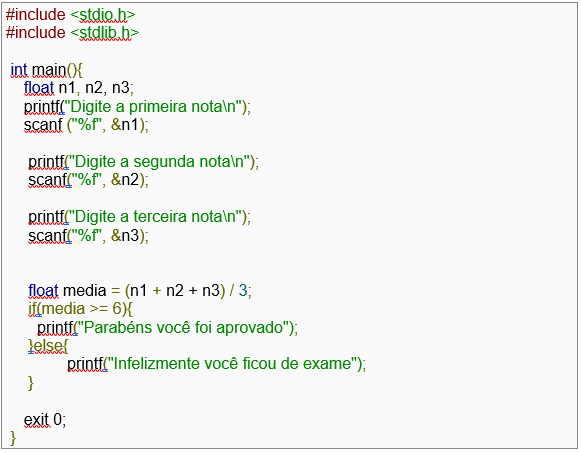
\includegraphics[width=0.9\textwidth]{figuras/Capturar.PNG}
\caption{Algoritmo em C que calcula a média de três notas}
\label{figuraEntrada}
\end{figure}

\par A ferramenta deve gerar uma saída como a abaixo.
\begin{figure}[h]
\centering
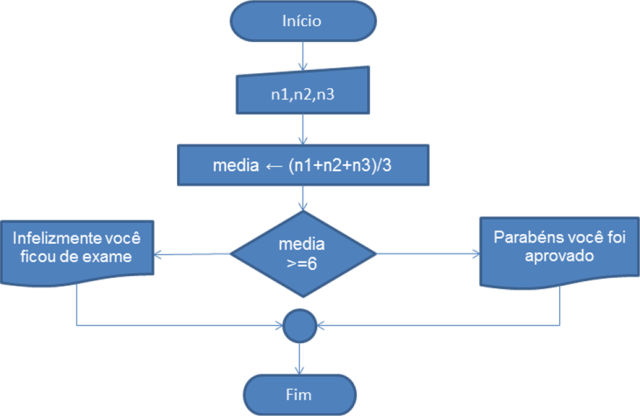
\includegraphics[width=0.9\textwidth]{figuras/fluxograma1.jpg}
\caption{Fluxograma representativo de saída}
\label{figuraSaida}
\end{figure}

\label{og}

\section{Objetivos Específicos}\label{oe}
Visando uma ferramenta totalmente gratuita e que faça a representação de uma estrutura lógica textual estruturada de forma gráfica, o objetivo deste trabalho é disposto em três etapas:
\begin{enumerate}

 \item Análise léxica e sintática necessária para separar e identificar estruturas de:
    \begin{enumerate}
    \item Entrada de dados
    \item Repetição
    \item Seleção de dados
    \item Blocos de instrução
    \item Funções
    \end{enumerate}
    
 \item Formalização das informações.
    \begin{enumerate}
    \item Após a identificação dos token (conjunto de caracteres com significado coletivo) --- REFERENCIA, seguir um modelo unificado e consolidado para representação visual das estruturas.
    \end{enumerate}
    
 \item Informações de saída.
    \begin{enumerate}
    \item Realizado o processamento e tradução dos dados é apresentado um fluxograma como especificado na etapa de formalização, assim como informações adicionais e explicativas (legendas, erros de sintaxe, erros léxicos e etc).
    \end{enumerate}
    
\end{enumerate}


\section{Justificativa}
Desenvolver a habilidade de escrever algoritmos é uma tarefa difícil, fato esse evidenciado em [DIJKSTRA 1982], onde explica-se que escrever um algoritmo necessita de um nível de raciocínio mais elevado que qualquer outra atividade. Pois também se trata de um trabalho de engenharia, devido a produção de ativos que devem seguir regras de qualidade e serem susceptíveis a apuração.\par
Assim a construção de uma ferramenta que explique esses conceitos de forma gráfica, ajudaria na compreensão de um conceito complexo e que constatadamente não possui entendimento rápido a partir de referências textuais (livros, artigos e demais formas de textuais).
\label{just}


\section{Método}
\par Tendo como um dos objetivos a acessibilidade, esta ferramenta deve ser capaz de ser executada tanto de forma online como offline. 
Com isto ela deve ser desenvolvida em uma versões web e desktop, sendo que a versão desktop poderá ser executada em sistemas Windows, Linux e Mac, visando alcançar o máximo de ambientes possíveis.
\par Com esta necessidade abordada a ferramenta deve ser desenvolvida em uma framework que adote o conceito de cross building também conhecido como cross compiler.
Pratica essa permite que um mesmo código seja utilizado para gerar uma aplicação executável em ambientes diferentes, para que o desenvolvimento ganhe produtividade e um bom grau de manutenibilidade. 
\par Assim as linguagens adotadas seram Html, css e js, através de um projeto NodeJs com React que na versão desktop será apresentado ao usuário por meio da biblioteca electron.
\par Para criação do fluxograma, os padrões especificados pelo diagrama de flowchart serão adotados, por se tratar de um modelo que possui estruturas representativas análogas as estruturas da lógica computacional estruturada textual, como:
\begin{itemize}
\item Entrada e saída de dados
\item Estruturas de repetição
\item Seleção de dados
\item Início e fim
\end{itemize}
\par Dentre outras que serão explanadas nos capítulos subsequentes.





%capítulo 2 - Fundamentação Teórica
\chapter{Analise Léxica}\label{fund}
Neste capítulo será descrito a base de conhecimento utilizada para o desenvolvimento do analisador léxico, assim como a importância desta fase dentro do projeto.
\section{O papel do analisador léxico}\label{label1}
A fase de análise léxica tem como objetivo identificar e separar em \textit{tokens}, trechos do código fonte em um padrão definido de acordo com linguagem do fonte.\par
Esta fase é responsável por ler os caracteres do código fonte agrupando-os em um fluxo de \textit{token}, onde cada \textit{token} representa uma serie de caracteres que possua um sentido lógico, como por exemplo, a identificação de uma palavra reservada da linguagem utilizada (if, while e etc), ou até mesmo um caractere de pontuação ou uma operação composta por mais de um caractere (==, \&\&, ; e etc).
Esta série de caracteres que formam um \textit{token} é chamada de lexema para aquele \textit{token}.\par
A identificação destes \textit{tokens} será de importância para complementar junto a analise sintática a construção da estrutura de uma arvore sintática, que será abordada nos capítulos subsequentes. Estrutura essa responsável por auxiliar na representação ao usuário, da ordem em que cada ação dentro do fonte será executada.\par
Estes \textit{token} gerados serão utilizados para identificar as regras de produção de expressões lógicas da linguagem.
Este analisador será construído para a linguagem C, afim de identificar algoritmos determinísticos. Isto é possível, dado que a linguagem C é uma linguagem livre de contexto, pois possui uma gramática simplificada.


\begin{citacao}
``Uma gramática descreve naturalmente a estrutura hierárquica de muitas construções das linguagens de programação. Por exemplo, um comando if-else, em C, possui a forma
if(expressão) comando else comando
Ou seja, o comando é uma concatenação da palavra-chave if, um parêntese à esquerda, uma expressão, um parêntese à direita, um comando, a palavra-chave else e um outro comando. Usando-se a variável expr a fim de denotar uma expressão a variável cmd para um comando (ou enunciado), esta regra de estruturação pode ser expressa como 
cmd -> if(expr) cmd else cmd
Onde seta pode ser lida como "pode ter a forma". Tal regra é chamada de produção. Numa produção, os elementos léxicos,
Como a palavra-chave if e os parênteses, são chamados de tokens. 
As Variáveis como expr e cmd representam sequências de tokens e são chamadas de não terminais.'' Pag 12 livro do dragão \cite{wang}
\end{citacao}

\begin{figure}[htp!]
\centering
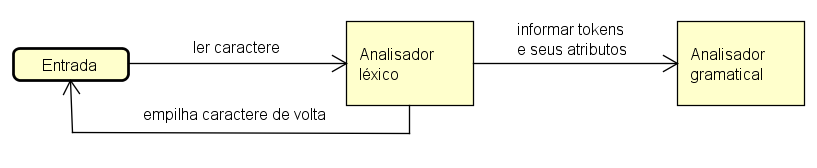
\includegraphics[width=\textwidth]{figuras/flxlexico.png}
\caption{Fluxo processual da análise léxica}
\label{figura1}
\end{figure}

\section{Especificação de tokens}\label{labelS1}
Expressões regulares são uma forma de especificar padrões. Cada padrão é correspondente ao respectivo conjunto de cadeias. Assim as expressões regulares serão responsáveis por um conjunto de cadeias de caracteres.
\par Uma expressão regular trata-se de uma notação que irá representar uma determinada sequência de caracteres. Este tipo de notação é empiricamente utilizado para validar entrada de dados ou fazer buscas e extração de informações em formato de texto.
\par Dentro da sintaxe de expressões regulares existem metacaracteres que podem ser classificados em quatro conjuntos:

\begin{itemize}
\item  Especificadores: determinam uma cadeia de caracteres a ser encontrada em uma determinada posição.
\item Quantificadores:  definem a quantidade de vezes que determinada sequência de caracteres irá se repetir.
\item Âncoras: Estabelecem a posição que determinada expressão irá ocorrer.
\item Agrupamento: Definem grupos ou alternativas possíveis.
\end{itemize}

\begin{table}[htbp!]
  \centering
    \caption{Especificadores}
      \begin{tabularx}{\textwidth}{|X|X|X|}
      \hline
      \textbf{metacaractere} &  \textbf{alcunha} & \textbf{significado} \\
      \hline
      . & curinga & qualquer caractere, exceto a quebra de linha. \\
      \hline
      [...] & conjunto & qualquer caractere incluído no conjunto.\\
      \hline
      [\textasciicircum{}...] & conjunto negado & qualquer caractere não incluído no conjunto.\\
      \hline
      \textbackslash{}d & dígito & o mesmo que [0-9]. \\
      \hline
      \textbackslash{}D & não-digito & o mesmo que [\textasciicircum{}0-9]. \\
      \hline
      \textbackslash{}s & branco & espaço, quebra de linha, tabs etc.; o mesmo que [\textbackslash{}t\textbackslash{}n\textbackslash{}r\textbackslash{}f\textbackslash{}v]. \\
      \hline
      \textbackslash{}S & não-branco & o mesmo que [\textasciicircum{}\textbackslash{}t\textbackslash{}n\textbackslash{}r\textbackslash{}f\textbackslash{}v]. \\
      \hline
      \textbackslash{}w & alfanumérico & o mesmo que [a-zA-Z0-9\_]. \\
      \hline
      \textbackslash{}W & não-alfanumérico & o complemento de \textbackslash{}w. \\
      \hline
      \textbackslash{} & escape & Anula o significado especial do metacaractere seguinte; por exemplo, \. representa apenas um ponto, e não o curinga. \\
      \hline
      \end{tabularx}
  \label{Tabela5}
\end{table}
% \pagebreak

\begin{table}[htbp!]
  \centering
    \caption{Quantificadores}
      \begin{tabularx}{\textwidth}{|X|X|X|}
      \hline
      \textbf{metacaractere} &  \textbf{significado} \\
      \hline
      \{n\} & exatamente n ocorrências \\
      \hline
      \{n,m\} & no mínimo n ocorrências e no máximo m.\\
      \hline
      \{n,\} & no mínimo n ocorrências.\\
      \hline
      \{,n\} & no máximo n ocorrências. \\
      \hline
      ? & 0 ou 1 ocorrência; o mesmo que {,1}. \\
      \hline
      + & 1 ou mais ocorrência; o mesmo que {1,}. \\
      \hline
      * & 0 ou mais ocorrências. \\
      \hline
      <<q>>? & modera qualquer um dos quantificadores acima. \\
      \hline
      \end{tabularx}
  \label{Tabela1}
\end{table}
% \pagebreak


\begin{table}[htbp!]
  \centering
    \caption{Âncoras}
      \begin{tabularx}{\textwidth}{|X|X|X|}
      \hline
      \textbf{metacaractere} &  \textbf{significado} \\
      \hline
      \textasciicircum{} & início do texto, ou de uma linha. \\
      \hline
      \A & início do texto.\\
      \hline
      \$ & fim do texto, ou de uma linha; não captura o \n no fim do texto ou da linha.\\
      \hline
      \textbackslash{}Z & fim do texto. \\
      \hline
      \textbackslash{}b & posição de borda, logo antes do início de uma palavra, ou logo depois do seu término; o mesmo que a posição entre \textbackslash{}W e \textbackslash{}w ou ambos . \\
      \hline
      \textbackslash{}B & posição de não-borda. \\
      \hline
      \end{tabularx}
  \label{Tabela2}
\end{table}
% \pagebreak

\begin{table}[htbp!]
  \centering
    \caption{Agrupamento}
      \begin{tabularx}{\textwidth}{|X|X|X|}
      \hline
      \textbf{metacaractere} &  \textbf{significado} \\
      \hline
      (...) & define um grupo, para efeito de aplicação de quantificador, alternativa ou de posterior a extração ou reuso. \\
      \hline
      ...|... & Alternativa; combina a expressão à direita ou à esquerda. \\
      \hline
      \textbackslash{}<<n>> & recupera o texto casado no enésimo grupo.\\
      \hline
      \end{tabularx}
  \label{Tabela3}
\end{table}
% \pagebreak

\pagebreak




\par As expressões serão utilizadas para especificar as regras de produção da linguagem C, utilizadas nos algoritmos a serem avaliados, com o fim de encontrar possíveis erros de léxicos e de quebrar as expressões com o intuito de agrupa-las formando uma cadeia de tokens que possuam um sentido lógico. Para a criação de uma estrutura que auxilie na representação gráfica do algoritmo analisado, algo como:

\begin{table}[htbp!]
  \centering
    \caption{Estrutura de auxílio, para geração de fluxograma}
      \begin{tabularx}{\textwidth}{|X|X|X|}
      \hline
      \textbf{Expressão Regular} &  \textbf{Token} & \textbf{Valor do atributo} \\
      \hline
      If & if & - \\
      \hline
      \{ & Startblock & - \\
      \hline
      \} & EndBlock & - \\
      \hline
      < & Relop & LT \\
      \hline
      <= & Relop & LE \\
      \hline
      == & Relop & EQ \\
      \hline
      != & Relop & NE \\
      \hline
      > & Relop & GT \\
      \hline
      > & Relop & GT \\
      \hline
      >= & Relop & GR \\
      \hline
      \end{tabularx}
  \label{Tabela4}
\end{table}
% \pagebreak

\pagebreak

\subsection{Reconhecimento de tokens}
\par Como citado acima uma gramática trata-se de um conjunto de regras definidas por expressões que representam uma cadeia de caracteres que podem ser classificados como terminais e não terminais. 
\par Terminais são classificados como uma sequência de caracteres que possam estar no início ou no fim de uma regra de produção, onde não possuam derivações dos mesmos. Terminais são caracterizados com palavras reservadas e delimitadores (if, else, while, \{).

\par Uma gramática é formada por regras de produção, que são constituídas de um conjunto de terminais e não terminais. Para que seja possível o reconhecimento de laços de repetição declaração de variáveis, dentre outras ações realizadas em um algoritmo, é necessário que sejam construídas regras produção que identifique estes passos. Está estrutura possuirá uma expressão regular e um token.

\par Considerando, fragmentos da gramática da linguagem C, serão identificadas estruturas como:

\begin{itemize}
\item Declaração de variáveis
\item Atribuição de valores
\item Comparações
\item Laços de repetição
\item Entrada e saída de dados
\item Declaração e utilização de funções
\end{itemize}


Assim o analisador léxico tem como proposta reconhecer algoritmos determinísticos não recursivos, escritos na liguagem C.



%capítulo 3 - Estudo de Viabilidade do Projeto proposto
\chapter{Fluxograma} \label{fluxograma}
\par Atualmente a disseminação do conceito lógico computacional estruturado textual, que envolve raciocínio lógico ou de sintaxe pesada, possui uma didática, utilizada empiricamente por professores da área, que tornam difícil o aprendizado do aluno. [Rocha 1991] e [Chen e Morris 2005]
\par Sabe-se que o ser humano possui mais habilidade em interpretar algoritmos em forma visual do que em formato texto. Isto se deve ao fato que o hemisfério esquerdo do cérebro processar informação oral e lógica, enquanto o hemisfério direito processa informação visual e espacial. Quando interpretarmos um texto o hemisfério direito não contribui de forma significativa para o aprendizado. [Da Silva 2001]
\par Assim a utilização de fluxogramas e outras formas de interpretação visual, de algoritmos lógicos computacionais textualmente estruturados, torna mais fácil o aprendizado, pois estimula ambos os lados do cérebro.
\par Neste sentido, este projeto tem como proposta, identificar e expor na forma de fluxogramas, a analise de algoritmos determinísticos não recursivos, escritos na linguagem C.

\begin{figure}[htp!]
\centering
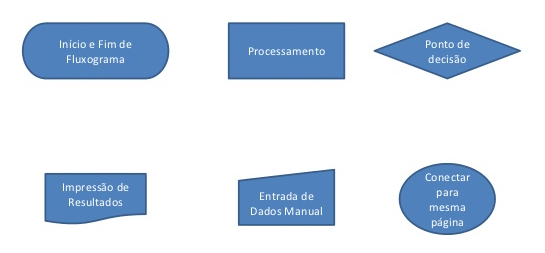
\includegraphics[width=\textwidth]{figuras/fluxograma2.png}
\caption{Formatos para geração de fluxograma}
\label{figura1}
\end{figure}

\begin{figure}[htp!]
\centering
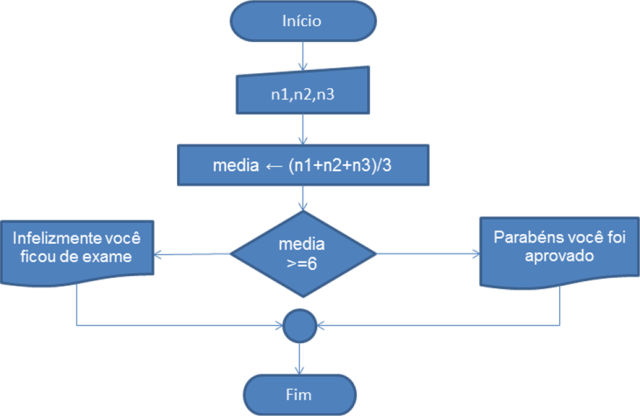
\includegraphics[width=\textwidth]{figuras/fluxograma1.jpg}
\caption{Exemplo de fluxograma final}
\label{figura2}
\end{figure}
% \chapter{ESTUDO DE VIABILIDADE} \label{estudo}

% Neste capítulo pretende-se mostrar por que o \textit{software} proposto será viável para áreas comerciais de qualquer ramo. As próximas seções falam sobre o mercado potencial, os benefícios, as oportunidades, as forças, as fraquezas, as ameaças e os concorrentes diferenciais.

% \section{Mercado potencial}

% \section{Benefícios}

% \section{Oportunidades}

% \section{Forças}

% \section{Fraquezas}


% \section{Ameaças}


% \section{Concorrentes Diferenciais}



%capítulo 4 - Descrição do Projeto
\chapter{DESCRIÇÃO DO PROJETO} \label{capitulo}

\section{Arquitetura}

\section{Descrição do Problema}

\section{Levantamento de Requisitos}

\subsection{Requisitos Funcionais e Não Funcionais}

As tabelas \ref{rf1} a seguir, apresentam um dos requisitos levantados para o sistema.

\begin{table}[htbp!]
\caption{nome da tabela}
\begin{center}
  \begin{tabularx}{\textwidth}{|c|X|c|c|c|}
      \hline
%multicolumn é a mesclagem da linha
      \multicolumn{4}{|l|}{\textbf{RF1: requisito}} & \multicolumn{1}{l|}{\textbf{Oculto:}}\\
      \hline
      \multicolumn{5}{|p{14cm}|}{\textbf{Descrição:} a descrição}\\
      \hline
      \multicolumn{5}{|c|}{\textbf{Requisitos não funcionais}}\\
      \hline
      \textbf{Nome} & \multicolumn{1}{c|}{\textbf{Restrição}} & \textbf{Categoria} & \textbf{Desejável} & \textbf{Permanente}\\
      \hline
      \textbf{NF 1.1} & requisito. &           & ( ) & (x)\\
      \hline
    \end{tabularx}
  \end{center}
  \label{rf1}
\end{table}


\subsection{Regras de Negócio}

\begin{table}[htbp!]
  \caption{Regras de Negócio}
  \centering
      \begin{tabularx}{\textwidth}{|l|X|X|}
    \hline
      \textbf{Regra} & \textbf{Nome} & \textbf{Descrição}\\
      \hline
      RN1 & Regra & Descrição.\\
      \hline
      RN2 & Regra & Descrição.\\
      \hline
      RN3 & Regra & Descrição.\\
      \hline
      RN4 & Regra & Descrição.\\
      \hline
      RN5 & Regra & Descrição.\\
      \hline
      RN6 & Regra & Descrição.\\
      \hline 
      \end{tabularx}
  \label{regra}
\end{table}


\subsection{Descrição dos Atores}


\section{Casos de Uso}


\subsection{Diagrama de Casos de Uso}


\subsection{Descrição dos Casos de Uso}

Modelo de tabela de descrição de um caso de uso.

\begin{table}[htpb!]
 \caption{Caso de Uso: Consultar Cliente}
  \begin{center}
    \begin{tabularx}{1.0\textwidth}{|X|}
    \hline
      \textbf{CSU1:} Consultar Cliente\\
      Este caso de uso descreve as funcionalidades para consultar um cliente no sistema.\\
      \hline
      \textbf{Atores:} Funcionário, Gerente\\
      \hline
      \textbf{Pré-Condição:} O usuário deverá estar logado no sistema.\\
      \hline
      \textbf{Pós-condição:} Não possui.\\
      \hline
      \textbf{Fluxo Principal:}
      \begin{enumerate}
        \item O caso de uso inicia quando o ator clicar na página consultar cliente.
        \item O sistema apresenta o botão Consultar para ser selecionado.
        \item O Ator clica no botão Consultar.
        \item O sistema realiza a busca dos dados informados na base de dados, retorna uma mensagem e então o caso de uso se encerra.
        \item Este caso de uso se encerra.
      \end{enumerate}\\
    \hline
      \textbf{Fluxo Alternativo (A1)}
      \begin{enumerate}
      \renewcommand{\labelenumi}{\alph{enumi}.}
        \item Se na etapa 2 do fluxo principal o ator informar que não deseja mais consultar um cliente,o passo seguinte é clicar no botão Cancelar e voltará para o passo nº 2, aguardando resposta do ator.
      \end{enumerate}\\
      \hline
      \textbf{Fluxo de Exceção (E1)}
      \begin{enumerate}
      \renewcommand{\labelenumi}{\alph{enumi}.}
        \item Dados não encontrados: na etapa 3 do CASO\#01 do fluxo principal, o sistema busca os clientes, informa mensagem de erro se não encontrar e posiciona o cursor do mouse no campo com erro.
      \end{enumerate}\\
    \hline
    \end{tabularx}
  \end{center}
  \label{dcu1}
\end{table}
\pagebreak


\section{Especificação da Análise}
\subsection{Diagrama de Pacotes}

\subsection{Diagrama de Classe}

\subsection{Diagrama de Entidade e Relacionamento}

\subsection{Dicionário de Dados}

Modelo de tabela de dicionário de dados.

%% ======================================Classe Funcionario=======================================================
\begin{table}[htp!]
\caption{Classe Funcionário}
\centering
\begin{tabularx}{\textwidth}{|X|X|X|}
\hline
\multicolumn{3}{|c|}{\textbf{Classe Funcionario}} \\
 \hline 
 \multicolumn{3}{|c|}{Contém as informações do funcionário} \\
 \hline
 \textbf{ATRIBUTO} & \textbf{TIPO} & \textbf{DESCRIÇÃO} \\
 \hline
 Id\_Cliente & Int & Identifica o funcionário \\
 \hline
 CPF & String & CPF do funcionário \\
 \hline
 Nm\_Funcionario & String & Nome do funcionário \\
 \hline
 Dt\_Nascimento & String & Data de nascimento do funcionário \\
 \hline
 Sexo & String & Sexo do funcionário \\
 \hline
 Cargo & String & Cargo do funcionário \\
 \hline
 Email & String & Email pessoal do funcionário \\
 \hline
 Nr\_Tel\_Cel & String & Número celular do funcionário \\
 \hline
 Nr\_Tel\_Res & String & Número residencial do funcionário \\
 \hline
 Usuario & Usuario & Usuário do funcionário \\
 \hline
 Endereco & Endereco & Endereço do funcionário \\
\hline
\end{tabularx}{}
\end{table}

\subsection{Diagrama de Atividades}

\subsection{Diagrama de Sequência}

\section{Descrição da implementação}




%capítulo 5 - Telas do protótipo pronto (TCC2)
\chapter{TELAS DO PROTÓTIPO} \label{telas}

Neste capítulo são apresentadas as telas do protótipo .....



%capítulo 6 - Validação do projeto
\chapter{VALIDAÇÃO E VERIFICAÇÃO} \label{val}

%capítulo 7 - Conclusão
\chapter{CONCLUSÃO}\label{conc}

\section{Considerações Finais}

\section{Dificuldades}

\section{Trabalhos Futuros}




%==============================================================================
%				  BIBLIOGRAFIA / REFERÊNCIAS
%==============================================================================
%Bibliografia com geração automática

%bibliografia é o nome do arquivo de bibliografia (bibliografia.bib)
\bibliography{bibliografia}{}

%abnt-alf = forma de apresentação da referência dentro do texto.
\bibliographystyle{abnt-alf}
%==============================================================================

%Bibliografia manual

\begin{thebibliography}{widest entry}
\bibitem[01]{wang} WANGENHEIM, Christiane Gresse Von; WANGENHEIM, Aldo Von. "Raciocínio Baseado em Casos", Curitiba, Atlas, 2003.
\bibitem[02]{Io02} Insercure org. \emph{The Network Explotation Tool and Security Scanner}. 2002. URL:\verb+http://www.insecure.org/nmap.+ Last Visited: 22/07/2002.
\end{thebibliography}




%==============================================================================
%				  ANEXOS (OPCIONAL)
%==============================================================================

\anexo

%Exemplo de capítulo que deve ser coloca em anexo
\chapter*{CÓDIGOS DESENVOLVIDOS}

Aqui você coloca os códigos desenvolvidos na criação do protótipo.
Um forma de inserir códigos de programação dentro do texto é:

\begin{lstlisting}
        #include 
        using namespace std;
 
        int main(int argc, char *argv[])
        {
            cout << "Ola mundo LaTeX" << endl;
        }
\end{lstlisting}

Outra possibilidade muito útil, é a importação do arquivo com o código fonte. Desta forma, se você modificar o código fonte, para atualizar o seu documento basta recompilar o arquivo LaTeX. O comando para importar código fonte para LaTeX é o seguinte:

\lstinputlisting{codigos/ola_mundo_latex.cpp}

Mais informações sobre esse assunto, entre no site: \verb+http://www.borges-solutions.com+
\verb+/inserindo-codigos-fonte-em-arquivos-latex/+



%Fim do documento
\end{document}